
\documentclass[aspectratio=169]{beamer}

\mode<presentation>
\usetheme{Boadilla}
\definecolor{NTHU1}{RGB}{127,16,132}
\definecolor{NTHU2}{RGB}{228,210,231}
\definecolor{blue}{RGB}{30,90,205}
\definecolor{red}{RGB}{213,94,0}
\definecolor{green}{RGB}{0,128,0}
\definecolor{charcoalgray}{RGB}{108,104,104}
\setbeamercolor{title}{fg=NTHU1}
\setbeamercolor{frametitle}{fg=NTHU1}
\setbeamercolor{block title}{bg=NTHU1, fg=white}
\setbeamercolor{block body}{bg=NTHU2}
\setbeamercolor{structure}{fg=NTHU1}
\setbeamercolor{item projected}{fg=white}
\setbeamercolor{item}{fg=NTHU1}
\setbeamercolor{subitem}{fg=NTHU1}
\setbeamercolor{section in toc}{fg=NTHU1}
\setbeamercolor{description item}{fg=NTHU1}
\setbeamercolor{caption name}{fg=NTHU1}
\setbeamercolor{button}{bg=NTHU1, fg=white}
\setbeamercolor{caption name}{fg=NTHU1}
\usepackage{graphics}
\usepackage{tikz}
\usepackage{amsmath}
\usepackage{bbm}
\usetikzlibrary{decorations.pathreplacing}
\usepackage{geometry}
\usepackage{booktabs}
\usepackage{bookmark}
\usepackage{multirow, makecell}
\usepackage{float}
\usepackage{fancyvrb}
\usepackage{caption}
\captionsetup[figure]{singlelinecheck = false, format= hang, justification=centering}
\captionsetup[subfigure]{singlelinecheck = false, format= hang, justification=raggedright}
\usepackage{subcaption}
\usepackage{adjustbox}
\usepackage{hyperref}
\usepackage{threeparttable}
\usepackage{appendixnumberbeamer} 
\usepackage[T1]{fontenc}
\usepackage[default]{lato} 
\usepackage{smartdiagram}
\smartdiagramset{
  back arrow disabled = true,
  module minimum width=1cm,
  module x sep = 3,
  uniform arrow color=true,
}
\usepackage{xcolor}
\usepackage{colortbl}
	\definecolor{light-gray}{gray}{0.99}

\newenvironment{wideitemize}{\itemize\addtolength{\itemsep}{10pt}}{\enditemize}
\newenvironment{wideenumerate}{\enumerate\addtolength{\itemsep}{10pt}}{\endenumerate}
\newenvironment{widedescription}{\description\addtolength{\itemsep}{10pt}}{\enddescription}
\hypersetup{
colorlinks=true,
linkcolor=NTHU1,
filecolor=green, 
urlcolor=blue,
}
\beamertemplatenavigationsymbolsempty
\setbeamercolor{author in head/foot}{bg=white, fg=NTHU1}
\setbeamercolor{title in head/foot}{bg=white, fg=NTHU1}
\setbeamercolor{date in head/foot}{bg=white, fg=NTHU1}
\setbeamercolor{section in head/foot}{bg=white, fg=NTHU1}
\setbeamercolor{headline}{bg=white}
\setbeamertemplate{footline}{
    \leavevmode%
    \hbox{%
        \begin{beamercolorbox}[wd=.333333\paperwidth,ht=2.25ex,dp=1ex,center]{date in head/foot}%
            \usebeamerfont{date in head/foot}%\insertdate
        \end{beamercolorbox}%
        \begin{beamercolorbox}[wd=.333333\paperwidth,ht=2.25ex,dp=1ex,center]{title in head/foot}%
            \usebeamerfont{title in head/foot}\insertshorttitle
        \end{beamercolorbox}%
        \begin{beamercolorbox}[wd=.333333\paperwidth,ht=2.25ex,dp=1ex,right]{date in head/foot}%
            \usebeamerfont{date in head/foot}\insertframenumber{}\hspace*{2em}
        \end{beamercolorbox}}%
        \vskip0pt%
    }
    %% May need to script the introduction!!!!!!
%\setbeamercolor{page number in head/foot}{fg=NTHU1}
\setbeamertemplate{section in toc}[sections numbered]
\setbeamertemplate{subsection in toc}{\leavevmode\leftskip=3em\rlap{\hskip-1.75em\inserttocsectionnumber.\inserttocsubsectionnumber}
\inserttocsubsection\par}
\setbeamerfont{subsection in toc}{size=\footnotesize}
%\setbeamertemplate{headline}{%
  %\begin{beamercolorbox}[ht=5.5ex]{section in head/foot}
    %\vskip2pt\insertnavigation{0.33\paperwidth}\vskip2pt
  %\end{beamercolorbox}%
%}
\newenvironment{transitionframe}{\setbeamercolor{background canvas}{bg=white}\setbeamertemplate{footline}{} \begin{frame}[noframenumbering]}{\end{frame}}


\makeatletter
\let\@@magyar@captionfix\relax
\makeatother


\title[]{Public Economics and Development} % Change this regularly
\subtitle[]{Week 11: Universal Income and Means-tested Welfare Programs Across the Globe }
\author[Lee]{Seung-hun Lee }
\institute[]{Taipei School of Economics\\ National Tsing Hua University}

\date[]{May 5th, 2026}

\begin{document}
\begin{transitionframe}
\titlepage
\end{transitionframe}


%%% Color slides for section headers: Use for colloquium version (The ones bewteen \iffals and \fi)

\section{Overview setup of the topic}

\begin{frame}
\frametitle{UBI and Targeted Transfers: Where in the World?}

\begin{columns}
\begin{column}{0.50\textwidth}
  \textbf{Universal Basic Income (UBI)}
  \begin{itemize}\setlength\itemsep{4pt}
    \item Kenya (GiveDirectly, 2017--): 20,000 recipients, 12-year horizon
    \item Finland (2017--18): 2,000 unemployed adults, 560 Euro/month
    \item Alaska Permanent Fund (universal dividend since 1982, \$1,000 - 2,000/year)
    \item Ongoing pilots in 20+ countries as of 2024 
    
  \end{itemize}
\end{column}
\begin{column}{0.48\textwidth}
  \textbf{Means-tested / Targeted Programs}
  \begin{itemize}\setlength\itemsep{4pt}
    \item 149 countries operate at least one social protection program 
    \item CCTs in 66+ LMICs; cover $\sim$760 million people 
    \item Social safety nets account for 1.5\% of GDP on average in LMICs
    \item Sub-Saharan Africa \& South Asia: lowest coverage ($<$20\% of poorest quintile)
  \end{itemize}
\end{column}
\end{columns}

\end{frame}



\begin{frame}
\frametitle{UBI vs.\ Targeted Transfers: Key Debates}

\begin{columns}
\begin{column}{0.48\textwidth}
  \textbf{Case for UBI}
  \begin{itemize}\setlength\itemsep{4pt}
    \item Eliminate exclusion errors
    \item Reduces stigma and administrative costs of targeting
    \item Provides a permanent income floor and insurance against shocks
    \item Evidence from pilots: no significant negative labor supply effects
  \end{itemize}
\end{column}
\begin{column}{0.48\textwidth}
  \textbf{Case for Targeted Transfers}
  \begin{itemize}\setlength\itemsep{4pt}
    \item Concentrating resources on the poor raises impact per dollar 
    \item CCTs generate human capital gains alongside income 
    \item UBI at adequate levels is fiscally unaffordable for most LMICs
    \item Political palatable for broader public
  \end{itemize}
\end{column}
\end{columns}

\medskip
\begin{block}{Central tension}
  \begin{itemize}\setlength\itemsep{3pt}
    \item[$\to$] \textbf{Universality} (coverage, low admin cost) vs.\ \textbf{Targeting} (sustainability, favor eligible poor)
    \item[$\to$] Neither dominates: optimal mix depends on fiscal/political constraint and objectives
  \end{itemize}
\end{block}
\end{frame}


\begin{frame}
\frametitle{Ongoing NIT experiment: Seoul Stepping Stone Income Project}
 Fun fact: I am part of the research team assessing this program \\ \medskip
Who is eligible?
\begin{itemize}\setlength\itemsep{3pt}
  \item Seoul residents with assets $\leq$ 326 million KRW ($\approx$ 236,000 USD)
  \item Cohort 1: income $\leq 50\%$ of standard median income; Cohort 2: $\leq 85\%$
  \item Coverage $\uparrow$, exclusion errors$\downarrow$, and generosity $\uparrow$ than existing programs
\end{itemize}\medskip
 
Transfers varies across income: Poorer households receive more
\begin{itemize}\setlength\itemsep{3pt}
\item Amount: half of the shortfall between current earnings and the income threshold 
  \item \textbf{50\% phase-out rate} vs.\ 70\% under existing program $\Rightarrow$ weaker labor disincentive
\end{itemize}\medskip
 
Experimental timeline: Assignment randomized among eligible applicants
\begin{itemize}\setlength\itemsep{3pt}
  \item Cohort 1 (484 treated, 1,039 control): treatment runs Jul 2022 -- Jun 2025
  \item Cohort 2 (1,100 treated, 2,488 control): treatment runs Jul 2023 -- Jun 2025
  \item Survey data collected twice per year; administrative data annually
\end{itemize}
\end{frame}




\begin{frame}
\frametitle{Increases in spending on essential and investment goods}
\input{tab1.tex}  
\end{frame}


\begin{frame}
\frametitle{Lower labor supply amongst recipients}  
\input{tab2.tex}
\end{frame}

\begin{frame}
\frametitle{Short-lived mental health effects amongst recipients}
\begin{figure}
  \centering
  \includegraphics[keepaspectratio, width=0.8\textwidth]{overall_mental.png}
\end{figure}
\end{frame}




\begin{transitionframe}
\frametitle{Roadmap for today}
\tableofcontents
\end{transitionframe}








\section{Theoretical motivation across different types of welfare programs}


\subsection{Moffit (2003): The Negative Income Tax and the Evolution of the US Welfare Policy}
\begin{transitionframe}
\begin{center}
  \begin{huge}
    \textcolor{NTHU1}{%
Moffit (2003):\\ The Negative Income Tax and the Evolution of the US Welfare Policy
    }
  \end{huge}
\end{center}
\end{transitionframe}


\begin{frame}
\frametitle{Q: How does negative income tax affect labor supply ? } 
Debate over labor supply effects across different welfare prgrams
\begin{itemize}\setlength\itemsep{3pt}
\item Positive income tax: Portion of income claimed as taxes and increase in income
\item Negative income tax (NIT): Send money back, but at decreasing rate as income rises
\begin{itemize}\setlength\itemsep{3pt}
\item Provide certain level of benefits event at zero income
\item But size of benefits reduced with more income
\end{itemize}
\item Early welfare designs had less interest in disincentives from welfare
\begin{itemize}\setlength\itemsep{3pt}
\item Generally benefits reduced by \$1 for each \$1 of earned income
\item NIT: benefites reduced by $< \$1$ per \$1 of earned income
\end{itemize}
\end{itemize}\medskip
This paper summarizes key components of NIT and analyzes its impact on labor supply
\begin{itemize}\setlength\itemsep{3pt}
\item Labor supply effect of NIT vs others
\item Provides studies on how some principles of NIT are adopted 
 \end{itemize}
\end{frame}






\begin{frame}
\begin{columns}
  \begin{column}{0.45\textwidth}
\frametitle{Friedman's version of NIT} 
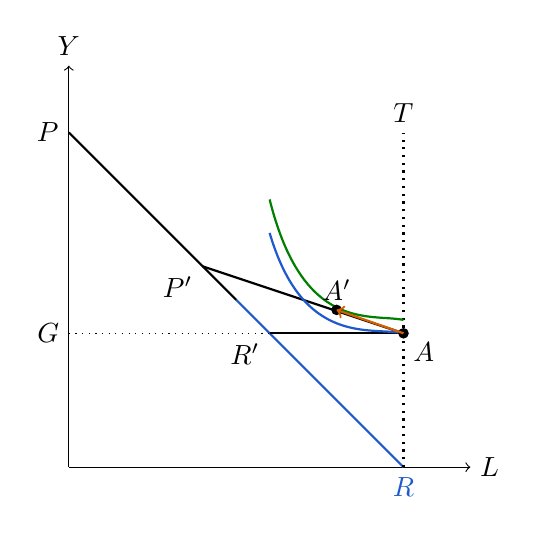
\begin{tikzpicture}[scale=0.85]
  \draw[->] (0,0) -- (6,0) node[right] {$L$};
  \draw[->] (0,0) -- (0,6) node[above] {$Y$};
  %% Original budget line
  \draw[thick, blue] (5,0) node[below] {$R$}-- (2.5,2.5) ;
  \draw[thick, black] (2.5,2.5) -- (0,5) node[left] {$P$};
  %% Post-tax budget line

  \draw[thick, black] (3,2) node[below left] {$R'$} -- (5,2);
  \draw[thick, black] (2,3) node[below left] {$P'$} -- (5,2);
  \draw[thick, dotted,black] (5,0) -- (5,5) node[above] {$T$};
  %% Compensated (Hicksian) budget line — same slope as post-tax, tangent to original IC

  %% Indifference curves (hand-drawn approximations as bezier)
\draw[thick, green] (3,4) .. controls (3.5,2) and (4.5,2.3) .. (5,2.2) ;

\draw[thick, blue] (3,3.5) .. controls (3.5,1.8) and (4.5,2.1) .. (5,2) ;

\draw[dotted, black] (0,2) node[left] {$G$} -- (3,2);
  %% Three points
  \filldraw[black] (5,2) circle (2pt) node[below right] {$A$};
  \filldraw[black]  (4,2.35) circle (2pt) node[above ] {$A'$};
  \draw[red, thick,->] (5,2) -- (4,2.35) ;



%  \filldraw[red]   (2.5,1) circle (2pt) node[below] {$B$};
  %% Braces
\end{tikzpicture}
\end{column}
\begin{column}{0.55\textwidth}

 Househod budget
\begin{itemize}\setlength\itemsep{3pt}
\item Earned income $Y$ + benefit $B$
\item $Y=w(T-L)=wl$ 
\item $B=\max\{0, G-tY\}$, where $t$ is tax on $Y$
\end{itemize}\medskip 
Minimum guaranteed income, with 100\% tax
\begin{itemize}\setlength\itemsep{3pt}
\item Guarantees $G$
\item Additional income fully taxed
\item Likely to choose no work (point $A$)
\end{itemize}\medskip
NIT with lower than 100\% tax rate
\begin{itemize}\setlength\itemsep{3pt}
\item Labor supply $\uparrow$ compared to above case
\item Targeting efficiency solely based on income (Friedman 1962)
\end{itemize}\medskip
\end{column}
\end{columns}
\end{frame}



\begin{frame}
\frametitle{Ambigious labor supply effect?} 
\begin{columns}
  \begin{column}{0.45\textwidth}
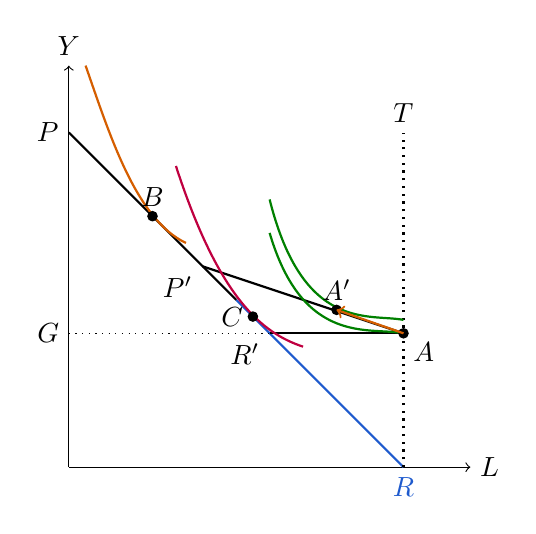
\begin{tikzpicture}[scale=0.85]
  \draw[->] (0,0) -- (6,0) node[right] {$L$};
  \draw[->] (0,0) -- (0,6) node[above] {$Y$};
  %% Original budget line
  \draw[thick, blue] (5,0) node[below] {$R$}-- (2.5,2.5) ;
  \draw[thick, black] (2.5,2.5) -- (0,5) node[left] {$P$};
  %% Post-tax budget line

  \draw[thick, black] (3,2) node[below left] {$R'$} -- (5,2);
  \draw[thick, black] (2,3) node[below left] {$P'$} -- (5,2);
  \draw[thick, dotted,black] (5,0) -- (5,5) node[above] {$T$};
  %% Compensated (Hicksian) budget line — same slope as post-tax, tangent to original IC

  %% Indifference curves (hand-drawn approximations as bezier)
\draw[thick, green] (3,4) .. controls (3.5,2) and (4.5,2.3) .. (5,2.2) ;
\draw[thick, green] (3,3.5) .. controls (3.5,1.8) and (4.5,2.1) .. (5,2) ;


\draw[thick, red] (0.25,6) .. controls (0.6,5) and (1,3.7) .. (1.75,3.35) ;

\draw[thick, purple] (1.6,4.5) .. controls (2.25,2.5) and (2.9,2) .. (3.5,1.8) ;

\draw[dotted, black] (0,2) node[left] {$G$} -- (3,2);
  %% Three points
  \filldraw[black] (5,2) circle (2pt) node[below right] {$A$};
  \filldraw[black]  (4,2.35) circle (2pt) node[above ] {$A'$};
  \draw[red, thick,->] (5,2) -- (4,2.35) ;
  \filldraw[black]  (1.25,3.75) circle (2pt) node[above ] {$B$};
  \filldraw[black]  (2.75,2.25) circle (2pt) node[left ] {$C$};
%  \filldraw[red]   (2.5,1) circle (2pt) node[below] {$B$};
  %% Braces
\end{tikzpicture}
\end{column}
\begin{column}{0.55\textwidth}

 Different labor supply responses
\begin{itemize}\setlength\itemsep{3pt}
\item Possible to increase $Y$ and $L$ ($C\to AP'$)
\item Possible to increase $L$ for lower $Y$ ($B\to AP'$)
\item Total change in labor supply is amibigous
\end{itemize}\medskip 
Other noticeable effects
\begin{itemize}\setlength\itemsep{3pt}
\item Cost effective targeting? Not always
\item More coverage cost with less labor possible if $B$ and $C$ re-optimize
\end{itemize}\medskip
Empiric evidence
\begin{itemize}\setlength\itemsep{3pt}
\item Labor $\downarrow$ in Seattle and Seoul ($t=0.7,0.5$)
\begin{itemize}
\item Except for single mothers (Seattle)
\item And those on previous welfare programs with higher $t$ (Seoul)+
\end{itemize}
\end{itemize}\medskip
\end{column}
\end{columns}
\end{frame}





\begin{frame}
\frametitle{Work requirments and categorical transfer systems} 
Work requirements definition
\begin{itemize}\setlength\itemsep{3pt}
\item  Cateogorize population to those who can and cannot work
\item Former receive benefits only if they satisfy minimum work hours (otherwise denied)
\item Latter given some guaranteed income, that phases out with earned income
\end{itemize}\medskip
Work requirement is at odds with NIT
\begin{itemize}\setlength\itemsep{3pt}
\item Against minimal government: need welfare bureaucracy to administer the program
\item Possibility to manipulate (mimick) into disability (where NIT purely based on income)
\end{itemize} \medskip
Proponents of work requirement
\begin{itemize}\setlength\itemsep{3pt}
\item Possible screening: Identify needy individuals who potentially benefit more
\item Work requirement as `ordeals' (Nichols, Zeckhause 1982)
\item Tagging and additional costs help identify the needy when true measure is unavailable
\end{itemize}
\end{frame}




\begin{frame}
\frametitle{Development of welfare in US: Welfare tax rates} 
Earned income tax credit (since 1996)
\begin{itemize}\setlength\itemsep{3pt}
\item Subsidy to earnings up to some point, which is phased out
\item Lower minimum guaranteed income
\item Also lower marginal tax rate on earned income (between 50-75\%)
\item Extended application of NIT: Wide rage of $t$ and eligibilty based on income
\item Heterogenous labor supply effect: Single mothers $\uparrow$, secondary earner work $\downarrow$
\end{itemize}\medskip
Other developments: Temporary assistance for needy families (TANF)
\begin{itemize}\setlength\itemsep{3pt}
\item Involved wthdrawal of benefits with additional income at varying rates
\item But also included components related to work requirements
\end{itemize}
\end{frame}

\begin{frame}
\frametitle{Development of welfare in US: Others} 
History of work requirement programs in US
\begin{itemize}\setlength\itemsep{3pt}
\item Growing element since 1970s: After NIT proposal by Nixon Admin was defeated
\item Minimum work hour started at 20 hrs per week (expanded to 30 hours)
\item Exemption on work requirement vary by state
\item Expenditure per recipient rose: Cost of regulating individual lives of welfare recipients
\item Did screen out those who have less need for support, reducing caseloads
\item Thus, room to create new programs to address different problems
\end{itemize}\medskip
Various means-tested programs
\begin{itemize}\setlength\itemsep{3pt}
\item Medicaid, Food stamps, Foster care, Supplemental Security Income etc
\item Screening based on non-income, ordeal-like measures
\end{itemize}
\end{frame}



\begin{frame}
\frametitle{Key messages} 
 
Takeaways
\begin{itemize}\setlength\itemsep{3pt}
\item Theorentical benefits of NIT not realized in some cases
\begin{itemize}\setlength\itemsep{3pt}
\item Ambigious labor supply effect
\item Gains from non-monetary screening mechanisms
\end{itemize}
\item Some developments is consistent with NIT: EITC, for instance
\item Others are not: Work requirement, means-tested programs
\item Still, NIT serves as theoretical framework to compare against other existing programs
\item Brought trade-offs between work incentives and support up front
\begin{itemize}\setlength\itemsep{3pt}
\item Also for marriage, education, child-bearing, among outcomes
\end{itemize}
\item Useful contribution to economic reasoning at public policy analysis
\end{itemize}\medskip
\end{frame}



\section{Studies on Universal Basic Income}

\subsection{Hanna, Olken (2018): Universal Basic Income versus Targeted Transfers: Anti-Poverty Programs in Developing Countries}
\begin{transitionframe}
\begin{center}
  \begin{huge}
    \textcolor{NTHU1}{%
Hanna, Olken (2018):\\ Universal Basic Income versus Targeted Transfers: Anti-Poverty Programs in Developing Countries
    }
  \end{huge}
\end{center}
\end{transitionframe}




\begin{frame}
\frametitle{Q: How do UBI and targeted programs address poverty?} 
Eradicating poverty worldwide is an important goal
\begin{itemize}\setlength\itemsep{3pt}
\item One of the SDGs articulated by the United Nations
\item While progress has been made, there are caveats
  \begin{itemize}\setlength\itemsep{3pt}
  \item Heavily driven by economic growth in India and China
  \item Even with future growth, still require substantial reduction in poverty
\end{itemize}
\item National-level transfers have an important role in this context
  \begin{itemize}\setlength\itemsep{3pt}
  \item Some based on targeting: Proxy means test and community based test
  \item Alternative is to reduce administratrive costs with UBI
\end{itemize}
\end{itemize}\medskip
This paper compares trade-offs observed across targeting and UBI
\begin{itemize}\setlength\itemsep{3pt}
  \item Examine how both programs are conducted in developing countries
  \item Investigates trade-offs based on evidence from Indonesia and Peru
\item Then draw implications on broader policy debate on redistribution
\end{itemize}
\end{frame}



\begin{frame}
\frametitle{Relationship between UBI and Income taxation problem} 
Design of UBI and taxation
\begin{itemize}\setlength\itemsep{3pt}
\item UBIs ultimately need to be financed via domestic taxation
\begin{itemize}\setlength\itemsep{3pt}
\item In general, external sources such as ODA takes up a very small share of the budget
\end{itemize}
\item Suppose UBI is given to all households
\item Households with income $y>0$ pay taxes progressive to their income to finance UBI
\end{itemize}\medskip
Trade-offs involved with UBI in developing countries
\begin{itemize}\setlength\itemsep{3pt}
\item Many individuals (80\% in some case) have reported income below tax thresholds
\begin{itemize}\setlength\itemsep{3pt}
\item Sometimes due to actually being poor, but also due to informal economies
\end{itemize}
\item Need to finance UBI from small group: High martinal tax rate for the few
\item Fewer overall funds $+$ Large labor disincentives on productive popualtion
\end{itemize}\medskip
\end{frame}

\begin{frame}
  \frametitle{Tax schedule with and without UBI, including tax exemption}
  \begin{figure}
    \centering
    \includegraphics[keepaspectratio, width=0.75\textwidth]{ho2018_f1.png}
  \end{figure}
\end{frame}

\begin{frame}
  \frametitle{Targeting in developing countries}
How targeting works when income is not perfectly observable
\begin{itemize}\setlength\itemsep{3pt}
\item Proxy means test based on census
\begin{itemize}\setlength\itemsep{3pt}
\item Door-to-door visits to examine visible assets and personal information
\item Rarely on self-reported basis (but people can misreport)
\end{itemize}
\item Use the information to predict household income
\begin{itemize}\setlength\itemsep{3pt}
\item Combine with other dataset collected for different purposes 
\item Regress poverty from other dataset with assets collected through census
\end{itemize}
\item Because of the \textit{predicted} nature, inclusion and exclusion errors exist
\end{itemize}\medskip
Other methods of targeting
\begin{itemize}\setlength\itemsep{3pt}
\item Community-based measures: Eligibility determined by community members
\begin{itemize}\setlength\itemsep{3pt}
\item Use localized information: Fill in gaps of standard measure but difficult to cross-compare
\end{itemize}
  \item Conditional transfers: Set conditions on receipt of benefits
  \begin{itemize}\setlength\itemsep{3pt}
\item Incentive effects (more education) targeting effects (may exclude very poor)
\end{itemize}
\end{itemize}
\end{frame}


\begin{frame}
\frametitle{Comparison of UBI and targeted transfers in Indonesia and Peru} 
Targeting program included in the study
\begin{itemize}\setlength\itemsep{3pt}
\item Peru: CCT for poor families (Juntos)
\item Indonesia: Nationwide UCT for poor household (BLT) 
\item Simulate targeting with assets from household data (2010-11) and varying thresholds
  \end{itemize}\medskip
Key findings on performance 
\begin{itemize}\setlength\itemsep{3pt}
\item Exclusion/inclusion error trade-off: 
\begin{itemize}\setlength\itemsep{3pt}
\item To reach 80\% of target beneficiaries, need to tolerate 22-31\% inclusion error
  \end{itemize}
\item Narrow vs wide targets on fixed budget 
\begin{itemize}\setlength\itemsep{3pt}
\item Transfers to per household fall as more people are allowed in
  \end{itemize}  
\item Welfare comparison
\begin{itemize}\setlength\itemsep{3pt}
\item Narrowly targeted programs perform better in terms of welfare
\item Large benefit-per-capita to the poorest of the poor
\item This holds even with large inclusion errors, but horizontal equity concerns may follow

  \end{itemize}
\end{itemize}
\end{frame}

\begin{frame}
  \frametitle{Error tradeoff and per household benefits}
  \begin{figure}
    \begin{subfigure}{0.4\textwidth}
      \centering
      \includegraphics[keepaspectratio, width=\textwidth]{ho2018_f2_1.png}
      \caption{Inclusion-exclusion error trade-off}
    \end{subfigure}
        \begin{subfigure}{0.57\textwidth}
      \centering
      \includegraphics[keepaspectratio, width=\textwidth]{ho2018_f2_2.png}
      \caption{Welfare amount per household}
    \end{subfigure}
  \end{figure}
\end{frame}

\begin{frame}
  \frametitle{Welfare and horizontal equity}
  \begin{figure}
    \begin{subfigure}{0.49\textwidth}
      \centering
      \includegraphics[keepaspectratio, width=\textwidth]{ho2018_f3_1.png}
      \caption{Social welfare across different simulations}
    \end{subfigure}
        \begin{subfigure}{0.49\textwidth}
      \centering
      \includegraphics[keepaspectratio, width=\textwidth]{ho2018_f3_2.png}
      \caption{Horizontal equity across different simulations}
    \end{subfigure}
  \end{figure}
\end{frame}



\subsection{Banerjee, Niehaus, Suri (2019): Universal Basic Income in the Developing World}
\begin{transitionframe}
\begin{center}
  \begin{huge}
    \textcolor{NTHU1}{%
Banerjee, Niehaus, Suri (2019):\\ Universal Basic Income in the Developing World
    }
  \end{huge}
\end{center}
\end{transitionframe}


\begin{frame}
\frametitle{Q: How does UBI affect individuals in developing countries?}
Raising income of the poor a pivotal goal in development economics and policy
\begin{itemize}\setlength\itemsep{3pt}
\item Universal basic income achieves this goal by design
\item Many funders and taxpayers worry about simply giving away money
\begin{itemize}\setlength\itemsep{3pt}
\item Worry about being too reliant on these transfers and/or wasting it away
\end{itemize}
\item More cost-effective way to raise income?
\begin{itemize}\setlength\itemsep{3pt}
\item Missing (credit) market, psychological burden of poverty more pressing and long-run
\item Large-scale infrastructural investment?
\item Perhaps a targeted income support does better, even in developing countries
\end{itemize}
\end{itemize}\medskip
This paper explores three questions on the effects of universal basic income
\begin{itemize}\setlength\itemsep{3pt}
\item What does individuals do with incremental income?
\item Would UBI unlock further economic growth?
\item Is it wise to give money to everyone, as oppoed to targeting?
\end{itemize}
\end{frame}



\begin{frame}
\frametitle{Where does incremental income go?} 
Where does the money for UBI come from?
\begin{itemize}\setlength\itemsep{3pt}
\item Repurposed foreign aid, re-allocating existing tax revenue, creating new taxes
\item Need to persuade many stakeholders
\begin{itemize}\setlength\itemsep{3pt}
\item Technocrats who design the policy
\item Tax payer who are also potential voters
\end{itemize}
\item Even a \textit{perceived} waste of UBIs (e.g. alcohol, drugs) reduces support for UBI
\end{itemize}\medskip
What do we know so far?
\begin{itemize}\setlength\itemsep{3pt}
\item UBI receipt reduced spending on temptation goods (alcohol, smoking etc)
\item Various positive effects on income, assets, food consumption, schooling, health etc
\begin{itemize}\setlength\itemsep{3pt}
\item These results, however, vary greatly across contexts
\item May reflect the feature that recipients have great autonomy with cash transfers
\item Imply that UBI may be suited for \textit{collective sets of} goals as opposed to \textit{particular} goal
\end{itemize}
\end{itemize}
\end{frame}



\begin{frame}
\frametitle{What we do not know about where money goes} 
Full-scale nationwide coverage is rare
\begin{itemize}\setlength\itemsep{3pt}
\item Coverage of the programs in developing countries is not 100\%
\item Broad coverage could induce general equilibrium effects
\begin{itemize}\setlength\itemsep{3pt}
\item Especially if there is a meaningful interaction between own and neighbor's income
\item If more in a given region is treated, could potentially affect market price and wages
\end{itemize}
\end{itemize}\medskip
Transfers to household vs transfers to each individual in the household
\begin{itemize}\setlength\itemsep{3pt}
\item Status quo: Typically goes to household head or mothers
\item Individualizing transfers may chage who decides how money is spent
\end{itemize}\medskip
No clear evidence of long-run effects of UBI
\begin{itemize}\setlength\itemsep{3pt}
\item Long-run UBI = Continuous inflow of income
  \item Savings may decrease ($\because$ less individual needed to smoothe consumption)
\item Increase tolerance for risk-taking
\end{itemize}
\end{frame}





\begin{frame}
\frametitle{Does UBI relax constraints placed on economic growth?} 
Financial constraints faced by the poor
\begin{itemize}\setlength\itemsep{3pt}
\item No credit market: Cannot save or borrow to make future investments
\item Underdeveloped insurance market: Shy away from making investments
\item UBI may not necessarily be the best tool to address these, but still useful
\begin{itemize}\setlength\itemsep{3pt}
\item But we do not exactly know which constraints bind for whom (and cannot target)
\item UBI, then, may serve as a catchall pro-growth policy in this context
\end{itemize}
\end{itemize}\medskip
What we find from various microcredit experiments and grant provisions
\begin{itemize}\setlength\itemsep{3pt}
\item Microcredit: Small loans to impoverished entrepreneurs w/o access to formal banks
\item On average, borrowers do not use loans to grow businesses
\item Heterogeneities: Those who already have business increase earnings (vs late starters)
\begin{itemize}\setlength\itemsep{3pt}
\item For those facing credit constraint, relaxing it through income provision helps
\item But not everyone faces credit constraint: UBI alone does not relax these
\end{itemize}
\end{itemize}
\end{frame}



\begin{frame}
\frametitle{Other constraints faced in developing countries} 
Lack of insurance markets in developing countries
\begin{itemize}\setlength\itemsep{3pt}
\item Evidence of more, high-risk \& high-return investments following subsidized insurance
\item Particularly among the more educated, and relatively wealthier population
\item Can UBI offset constraints from uninsured risk?
\begin{itemize}\setlength\itemsep{3pt}
\item Could potentially help meet basic needs, which is required prior to taking risks
\item Very little empirical research
\end{itemize}
\end{itemize}\medskip
Constraints from psychological factors
\begin{itemize}\setlength\itemsep{3pt}
\item Poverty leads to costs in mental bandwidth
\item Graduation programs with training increase earnings/assets through aspirations
\begin{itemize}\setlength\itemsep{3pt}
\item But limited impacts on those who had very little to begin with
\end{itemize}
\item UBI could relax mental toll by reducing worries about making ends meet
\begin{itemize}\setlength\itemsep{3pt}
\item Positive effects on mental health, decreases in suicides
\item But long-run effects not yet consolidated
\end{itemize}
\end{itemize}
\end{frame}


\begin{frame}
\frametitle{Better to target or not?} 
Measuring poverty in developing countries
\begin{itemize}\setlength\itemsep{3pt}
\item Mostly on household poverty, as opposed to individual poverty
\item Inclusion/exclusion errors: What if poorest individuals are not from poorest hhs?
\item Costs of targeting: High especially in presence of informal economies
\item Difficult to update poverty measure: Hard to catch changes in distribution of poverty
\item Requires functioning bureaucracies: Otherwise opportunities for corruption
\end{itemize}\medskip
Can UBI schemes do better? Above problems may also exist here
\begin{itemize}\setlength\itemsep{3pt}
\item Still need universal identification system to prevent double counting and exclusion
\begin{itemize}\setlength\itemsep{3pt}
\item Incurs large one-time investment
\end{itemize}
\item Still face problem of accurately measuring poverty
\item Also require capable bureaucracies to implement
\end{itemize}
\end{frame}


\begin{frame}
\frametitle{Key messages from the paper} 
Studies on the UBI (and other targeting programs) are in evolving phase
\begin{itemize}\setlength\itemsep{3pt}
\item Many effects are very heterogeneous across different groups of individuals
\item This makes generalizing the effects of these programs difficult
\item So far, UBI does have positive measure across many measures
\item But if the fix is targeting a \textit{particular} measure, UBI may not be first-best
\begin{itemize}\setlength\itemsep{3pt}
\item Health, education investments, consumption, lumpy investments
\item But if a targeting a particular problem, better to design programs specific for that purpose
\end{itemize}
\item So is it better to switch existing programs to a single transfer?
\begin{itemize}\setlength\itemsep{3pt}
\item If so, people will buy these services on the market with the given money 
\item But private sector (markets) for these goods and services do not exist in many places
\item Thus, this paper is NOT about advocating switch from existing programs to cash transfers
\end{itemize}
\end{itemize}\medskip
\end{frame}



\section{Targeted transfers: A Look into Earned Income Tax Credit Program}
\subsection{Eissa, Liebman (1996): Labor Supply response to Earned Income Tax Credit}
\begin{transitionframe}
\begin{center}
  \begin{huge}
    \textcolor{NTHU1}{%
Eissa, Liebman (1996):\\ Labor Supply response to Earned Income Tax Credit
    }
  \end{huge}
\end{center}
\end{transitionframe}



\begin{frame}
\frametitle{Q: How does expanding EITC affect labor supply?} 
Traditional welfare for children reduced benefits 1-for-1 with additional income
\begin{itemize}\setlength\itemsep{3pt}
 \item Theory and evidence point to decline in labor force participation
 \item Reforms in the US around 1990s refunds credit in excess of tax liability
\begin{itemize}\setlength\itemsep{3pt}
\item Thus, welfare benefits decrease less than \$1 for each \$ of additional income
\end{itemize}
\item There are those who predict that EITC will enourage labor supply
\item But this is contentious: Many recipients are in phase-out or constant credit region
\end{itemize}\medskip
This paper documents classical evidence of labor supply effects of expanded EITC
\begin{itemize}\setlength\itemsep{3pt}
  \item Leverages a major welfare reform in 1986 (TRA86)
  \item Comparing single women with children to single women with no children
  \item Investigates changes in labor force particpation and hours worked
  \end{itemize}
\end{frame}



\begin{frame}
\frametitle{Eligibility and identification}
Who is eligible and how much are they credited?
\begin{itemize}\setlength\itemsep{3pt}
    \item Nonzero earned income (labor, business income)
    \item Adjusted gross income and earned income below specific amount (\$28,495 in 1996)
    \item Must have children, grandchildren, stepchild, or foster child below age 19 or disabled
    \item Credit and liability for households with children of 2
    \begin{itemize}\setlength\itemsep{3pt}
    \item Phase in rate of 40\% for first \$8,890 (max credit \$3,356), constant until \$ 11,610
    \item Phase out from \$11,610 at 21.06\% rate - no longer eligible at \$28,495
\end{itemize}    
\end{itemize}\medskip

Identification uses DID with the expansion of EITC in 1987 (passed in 1986)
\begin{itemize}\setlength\itemsep{3pt}
  \item Rise in phase-in credit rate, maximum credit, reduction in phase-out rate
  \item Also came in with other increased deductions that reduced tax burdens
    \item Single women with children (treated) vs single women without children (control)
    \begin{itemize}\setlength\itemsep{3pt}
    \item Largest group eligible for EITC vs simliar characteristics but unaffected by treatment
    \item No need to worry about joint labor supply decisions  
  \end{itemize}

  \end{itemize}
\end{frame}

\begin{frame}
  \frametitle{Increased labor force participation among single women w/ children}
  \begin{figure}
    \centering
    \includegraphics[keepaspectratio, width=0.8\textwidth]{el1996_t1.png}
  \end{figure}
\end{frame}


\begin{frame}
  \frametitle{Also confirmed through probit regression}
  \[
  \Pr(\text{lfp}_{it}=1)=\Phi(\alpha+\gamma_0\text{Kids}_i+\gamma_1\text{Post86}_t+\gamma_3\text{Kids}_i\times\text{Post86}_t + \beta Z_{it} )
  \]
  \input{el1996_t2.tex}
\end{frame}

\begin{frame}
  \frametitle{Expected effects on working hours}
  \begin{columns}
    \begin{column}{0.525\textwidth}
\centering
\includegraphics[keepaspectratio, width=\textwidth]{el1996_f1.png}
    \end{column}
    \begin{column}{0.475\textwidth}
      Region A ($0\leq y \leq 14,081$): Ambigous
      \begin{itemize}\setlength\itemsep{3pt}
        \item Income and substitution mixed
        \item Strength of effect depends on $y$
      \end{itemize}\medskip 
      Region B ($14,081 \leq y \leq 25,000$): Hours $\downarrow$
      \begin{itemize}\setlength\itemsep{3pt}
        \item Marginal tax rate per additional $y\uparrow$
        \item Some just above max credit may reduce hours (and $y$) to receive EITC
      \end{itemize}\medskip
      Region C: Likely unaffected
        \begin{itemize}\setlength\itemsep{3pt}
        \item High-earners
        \item May not be worth it to reduce $y$ 
      \end{itemize}
    \end{column}
  \end{columns}
\end{frame}


\begin{frame}
  \frametitle{Limited working hour changes among those already working}
  \begin{figure}
    \centering
    \includegraphics[keepaspectratio, width=0.95\textwidth]{el1996_t3.png}
  \end{figure}
\end{frame}


\begin{frame}
\frametitle{Key findings and discussion} 
Other key findings
\begin{itemize}\setlength\itemsep{3pt}
  \item Increase in labor supply of treated group not explained by different long-run trends
  \item Neither do other changes in late 80s (Other programs \& state-wide unemployment) 
  \item Large particpation increase but minimal labor hour changes
\begin{itemize}\setlength\itemsep{3pt}
  \item Pretty common in the literature: Work hour usually fixed by contract
\end{itemize}
\end{itemize}\medskip
Discussion on the overall EITC impacts
\begin{itemize}\setlength\itemsep{3pt}
    \item Labor supply changes are only part of the evaluation
    \item How much labor supply changes/distortion exists \textit{compared to other programs} matters
    \item What people do with the extra money matters: Expenditure, savings, assets etc
    
\end{itemize}
\end{frame}




\subsection{Kleven (2024): The EITC and the Extensive Margin: A Reappraisal}
\begin{transitionframe}
\begin{center}
  \begin{huge}
    \textcolor{NTHU1}{%
Kleven (2024):\\ The EITC and the Extensive Margin: A Reappraisal
    }
  \end{huge}
\end{center}
\end{transitionframe}

\begin{frame}
\frametitle{Q: Are the previous studies on EITC correct on labor supply effects?}
Shifts in assisting the poor to the \textit{working} poor
\begin{itemize}\setlength\itemsep{3pt}
\item Number of recipients of EITC = 30 times the number of other welfare
\item Expansion of EITC based on observation that labor supply at extensive margin $\uparrow$
\item Traditional welfare, on the ohter hand, blamed for labor disincentives
\end{itemize}\medskip
This paper reassess previous labor supply evidence on EITC
\begin{itemize}\setlength\itemsep{3pt}
\item Long-run analysis of all EITC reforms since 1975
\item Employs event-study approach: Fuller characterization of dynamic effects
\item Tests previous findings with different empirical models
\item Distinguishes pure EITC effects from confounding factors 
\item While focusing on the same population: Single women with and without children
\end{itemize}
\end{frame}


\begin{frame}
\frametitle{Data on EITC reforms studied in this period}
EITC and welfare reforms
\begin{itemize}\setlength\itemsep{3pt}
\item Federal: `75, `86 (studied in previous paper), `90, `93, `09
\begin{itemize}\setlength\itemsep{3pt}
\item `75 (EITC introduction) is the largest, followed by `93 expansion
\end{itemize}
\item State: 30 states introduced EITC supplements in `84-`18
\item Others: Various state-level reforms culminated to nationwide-level at `92-`96
\begin{itemize}\setlength\itemsep{3pt}
\item Introduction of Temporary Assistance for Needy Families (Families)
\item Time limits and work requirements, but benefits strictly increasing in children 
\end{itemize}
\end{itemize}\medskip
Data and empirical strategy
\begin{itemize}\setlength\itemsep{3pt}
\item Demographics and socioeconomic status gathered from Current Population Survey 
\item Treatment group will be single women with children
\item But also analyze heterogeneity of EITC effects across following categories
\begin{itemize}\setlength\itemsep{3pt}
\item Heterogeneity by predicted earnings based on observables
\item Education, \# of children, age of youngest children, race, and state
\end{itemize} 
\end{itemize}
\end{frame}

\begin{frame}
  \frametitle{Changes in EITC setup over time (Max credit)}
  \begin{figure}
    \centering
    \includegraphics[keepaspectratio, width=0.9\textwidth]{k2024_f1.png}
  \end{figure}
\end{frame}

\begin{frame}
  \frametitle{Limited labor supply changes except for `92-`96}
  \begin{figure}
    \centering
    \includegraphics[keepaspectratio, width=0.8\textwidth]{k2024_f2.png}
  \end{figure}
\end{frame}

\begin{frame}
  \frametitle{...also the case when event studies are applied}
  \begin{figure}
    \centering
    \includegraphics[keepaspectratio, width=1\textwidth]{k2024_f3.png}
  \end{figure}
  \begin{footnotesize}
    Note: This pattern holds when only those with bottom half of predicted earnings are included (Fig 6 in text)
  \end{footnotesize}
\end{frame}


\begin{frame}
  \frametitle{Effects mostly driven by state-level waiver reforms}
  \begin{figure}
    \centering
    \includegraphics[keepaspectratio, width=0.8\textwidth]{k2024_f4.png}
  \end{figure}
  \begin{footnotesize}
    Net out waiver reform states and control for macroeconomy (unemployment) $\to$ Event-study for `96 reform?
  \end{footnotesize}
\end{frame}



\begin{frame}
  \frametitle{Other findings and discussion}

So what does this imply about findings on EITC?
\begin{itemize}\setlength\itemsep{3pt}
\item Many econometric specifications only capture short-run effects
\item Treatment status based on fertility may not be the best approach
\item Ignoring contemporaneous effects may mask effects of potential confounders
\end{itemize}\medskip
So does this mean that EITC is ineffective? Not necessaarily
\begin{itemize}\setlength\itemsep{3pt}
\item Effects on other outcomes (health, household finances) still studied
\item Ultimately depends on redistribution
\begin{itemize}\setlength\itemsep{3pt}
\item Is it financed by those who are able to finance them?
\item Are working poor receiving higher consideration compared to the average?
\end{itemize}
\item Optimality depends on holistic set of goals, not just labor supply responses
\end{itemize}
\end{frame}

\begin{frame}
\frametitle{Unanswered questions}
Overall effect on reducing extreme poverty
\begin{itemize}\setlength\itemsep{3pt}
\item Conflicting findng on labor supply, a proxy for long-run self-sustenance
\item Many household finance outcomes still being explored
\item Implementation of graduation programs and studies on their effects underway
\begin{itemize}\setlength\itemsep{3pt}
\item Time-limited, structured programs to get ultra-poor out of poverty
\item Bundle transfers with job training, asset accumulation, household finance
\item Aim for eventual self-sustenance and decreased reliance on welfare programs
\end{itemize}
\end{itemize}\medskip

Room for further research on other aspects
\begin{itemize}\setlength\itemsep{3pt}
\item How much does implementation (not program design) matter?
\begin{itemize}\setlength\itemsep{3pt}
\item Many incidences of incapable and/or corruptible agents
\item How much of the (lack of) effect is attributable to poor implementation vs poor design?
\item Can implementation of technology reduce administrative burden, easing implementation?
\end{itemize}
\item How to implement such programs while minimizing political distate?
\end{itemize}
\end{frame}



%%%%%%%%%%%
\end{document}
